\section{Theory}

Previously, we have worked with \textbf{combinational circuits}, for which the output
is determined completely by the existing state of the inputs. There is no “memory,” in these circuits. Circuits that store some history make it possible to construct counters, arithmetic accumulators, and circuits that generally do one thing after another. Such circuits that remember their current output or state are often called \textbf{sequential logic circuits}.

The basic principle of memory is the concept of \textbf{feedback}.

\begin{figure}[H]
    \centering
    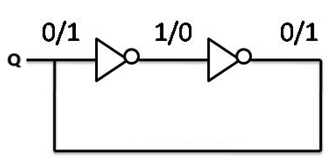
\includegraphics[width=0.50\columnwidth]{images/feed.png}
    \caption{Simplest realization of feedback circuit}
    \label{feedback}
\end{figure}

In Fig. \ref{feedback}, if Q happens to be 1 (or 0), it will always be 1 (or 0). While this circuit is of not much use, we use this principle in realizing the most basic form of a sequential circuit which is the \textbf{flip-flop}. A flip-flop circuit has two outputs, one for the normal value and one for the complement value of the stored bit.

\subsection*{RS Flip-Flop}
The simplest form of a flip-flop circuit, it can be constructed using either \verb|NAND| or \verb|NOR| gates.

An RS flip-flop circuit using \verb|NOR| gates is shown below. The inputs R and S refer to \verb|SET| and \verb|RESET| respectively.

\begin{itemize}
    \item Assume that $S=1$ and $R=0$. The output of the bottom \verb|NOR| gate is $Q'=0$. So, both inputs to the top NOR gate, $Q=1$. Hence, the input combination leads to the flip-flop being \textbf{set} to $Q=1$ and $Q'=0$.
    \item Similarly, if $S=0$ and $R=1$, $Q=0$ and $Q'=1$, i.e. the flip-flop is \textbf{reset}.
    \item Assume the flip-flop is in the set state. Now if one changes S to 0, the output still remains the same ($Q=1$ and $Q'=0$). Similarly, if the flip-flop is in the reset state and we change R to 0, the output still remains the same ($Q=0$ and $Q'=1$). This means in the state $S=0, R=0$, the circuit retains its previous output, also known as the \textbf{hold} state.
    \item When both $R=1$ and $S=1$, both outputs are no longer compliments of each other. Since it is impossible to predict which output will go to 1, this is an invalid state making it one of the main disadvantages of the RS flip-flop. 
\end{itemize}

\begin{figure}[H]
    \centering
    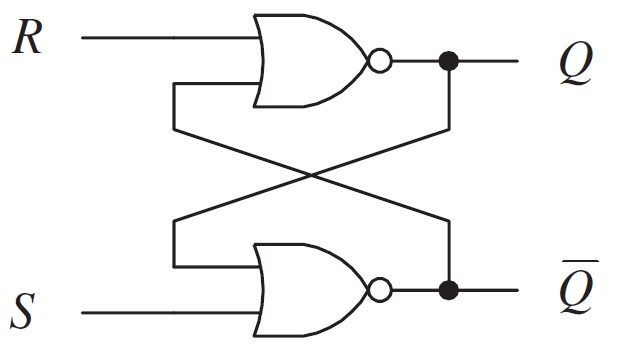
\includegraphics[width=0.50\columnwidth]{images/rs.jpg}
    \caption{Circuit diagram of an RS flip-flop}
    \label{1}
\end{figure}

\begin{table}[H]
    \centering
    \begin{tabularx}{0.75\columnwidth}{|Y|Y|Y|Y|Y|}\hline
        $R$ & $S$ & $Q$ & $Q'$ & Remark \\ \hline
        0 & 0 & $Q$ & $Q'$ & \verb|HOLD| \\ 
        0 & 1 & 1 & 0 & \verb|SET| \\ 
        1 & 0 & 0 & 1 & \verb|RESET| \\ 
        1 & 1 & - & - & Invalid \\ \hline
    \end{tabularx}
    \caption{Characteristic Table for an RS Flip-Flop}
\end{table}

\paragraph*{\textbf{Switch Debouncing:}}
A useful example of this flip-flop is the debounce circuit. Suppose a
piece of electronics is to change state under the action of a mechanical switch. When this
switch is moved from position S to R ($S=0, R=1$). When the switch is closed, the two contacts actually separate and reconnect, typically 100s of times over a period of about a millisecond. It is desirable that the electronics should respond to the first contact and then remain stable, rather than switching back and forth as the circuit makes and breaks. 

This is achieved by RS flip-flop which is reset to $Q=0$ by the first signal $R=1$ and remains in a fixed state until the switch is moved back to position S, when the signal $S=1$ sets the flip-flop to $Q=1$.

\begin{figure}[H]
    \centering
    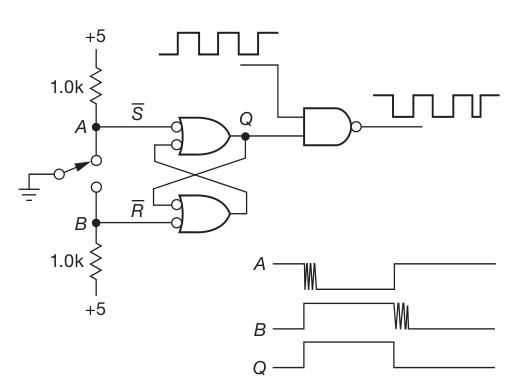
\includegraphics[width=0.80\columnwidth]{images/debounce.png}
    \caption{An example of an SR flip-flop switch debouncer.}
\end{figure}

% =====================================================================================
\subsection*{Gated or Clocked RS Flip-flop}
By connecting an AND gate in series with each input terminal of the RS NOR Flip-flop, we can construct a Gated RS Flip-flop. This extra conditional input is called an \textit{Enable} (EN) input.
When the $EN = 0$, the outputs of the two AND gates are also at 0, regardless of the inputs S and R, hence latching the two outputs $Q$ and $Q'$ into their last known state. When the $EN = 1$, the circuit acts like a normal RS bistable
flip-flop.

EN input can also be connected to a clock timing signal adding
clock synchronisation to the flip-flop creating what is sometimes called a
\textit{Clocked RS Flip-flop}.

\begin{figure}[H]
    \centering
    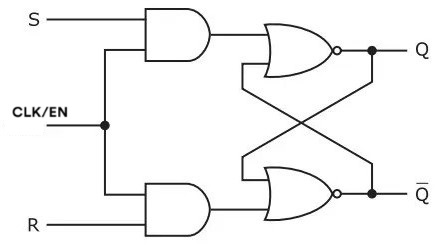
\includegraphics[width=0.60\columnwidth]{images/gatedrs.jpg}
    \caption{Circuit diagram of a gated RS flip-flop}
    \label{2}
\end{figure}

\begin{table}[H]
    \centering
    \begin{tabular}{|c|c|c|c|c|}\hline
        $Q_N$ & $R$ & $S$ & $Q_{N+1}$ & Remark \\ \hline
        0 & 0 & 0 & 0 & \verb|HOLD| \\ 
        0 & 0 & 1 & 0 & \\ 
        0 & 1 & 0 & 1 &\\ 
        0 & 1 & 1 & - &Indeterminate \\ 
        1 & 0 & 0 & 1 &\verb|HOLD|\\ 
        1 & 0 & 1 & 0 &\\ 
        1 & 1 & 0 & 1 &\\
        1 & 1 & 1 & - & Indeterminate \\ \hline
    \end{tabular}
    \caption{Characteristic Table for a Gated RS Flip-flop}
\end{table}
% =====================================================================================
\subsection{D Flip-flop}
The D flip-flop has only a single data input D. This D input and its inverse are connected to S and R inputs respectively. Thus, this eliminates the undefined state of $R=S=1$ seen in case of RS flip-flops.
A D-flip flop has a second input called Enable, EN, to allow the flip-flop to
be in a holding state, as seen in the circuit diagram.

\begin{figure}[H]
    \centering
    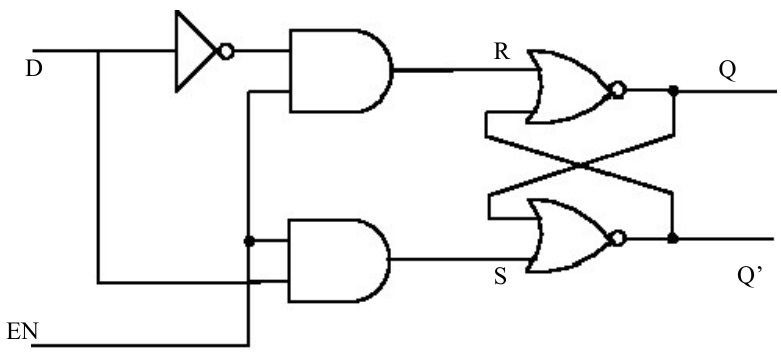
\includegraphics[width=0.60\columnwidth]{images/d.jpg}
    \caption{Circuit diagram of a D flip-flop}
    \label{3}
\end{figure}

\begin{itemize}
    \item When $EN=1$, $S=D$ and $R=D'$. Hence the output $Q$ follows $D$.
    \item When $EN=0$, irrespective of $D$, the most recent state is held. 
\end{itemize}

\begin{table}[H]
    \centering
    \begin{tabular}{|c|c|c|c|}\hline
        $Q_N$ & $D$ & $Q_{N+1}$ \\ \hline
        0 & 0 & 0 \\ 
        0 & 1 & 1 \\ 
        1 & 0 & 0 \\ 
        1 & 1 & 1 \\ \hline
    \end{tabular}
    \caption{Characteristic Table for a D Flip-flop, with $EN=1$ (hence no HOLD state).}
\end{table}


% =====================================================================================
\subsection*{JK Flip-flop}
The JK flip flop, named after Jack Kilby who invented it is
the most commonly used flip-flop.
It is basically a gated SR flip-flop with the addition of a clock input circuitry that prevents the illegal or invalid output condition that can occur when both inputs $S=R=1$. Due to this additional clocked input, a JK flip-flop has four possible output combinations, $1$, $0$, \textit{no change} and \textit{toggle}.

Note that in the following circuit diagram NAND gates are used instead of NOR gates.

\begin{figure}[H]
    \centering
    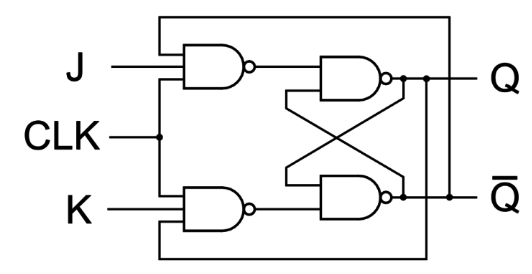
\includegraphics[width=0.70\columnwidth]{images/jk.png}
    \caption{Circuit diagram of a JK flip-flop}
    \label{4}
\end{figure}

The two 2-input AND gates of the gated SR bistable have now been replaced by two 3-input NAND gates with the third input of each gate connected to the outputs at Q and Q. This cross-coupling allows the previously invalid condition of $S=R=1$ state to be used to produce toggle action as the two inputs are now interlocked. We can summarize its operation as follows.

\begin{itemize}
    \item Assume the clock signal is 1. If $J=1$ and $K=0$, it behaves as a typical SR latch, i.e. $Q=1$ and $Q'=0$. Similarly for $J=0$ and $K=1$, $Q=0$ and $Q'=1$.
    \item If both $J=K=0$, then it remains in the same state as it was before i.e. the \verb|HOLD| state.
    \item If both $J=K=1$, the flip-flop changes state whenever a clock
    pulse occurs; i.e., the clock pulse toggles the flip-flop again and again until the Clk goes to 0. This is called is \textit{race-around condition} (Fig. \ref{race0}) and is undesirable, which is eliminated by an improvised form of this flip-flop as discussed next.
\end{itemize}

\begin{table}[H]
    \centering
    \begin{tabular}{|c|c|c|c|c|}\hline
        $Q_N$ & $J$ & $K$ & $Q_{N+1}$ & Remark \\ \hline
        0 & 0 & 0 & 0 & \verb|HOLD| \\ 
        0 & 0 & 1 & 0 & \\ 
        0 & 1 & 0 & 1 &\\ 
        0 & 1 & 1 & 1 & \verb|TOGGLE| \\ 
        1 & 0 & 0 & 1 & \verb|HOLD|\\ 
        1 & 0 & 1 & 0 &\\ 
        1 & 1 & 0 & 1 &\\
        1 & 1 & 1 & 0 & \verb|TOGGLE| \\ \hline
    \end{tabular}
    \caption{Characteristic Table for a JK Flip-flop}
\end{table}

\begin{figure}[H]
    \centering
    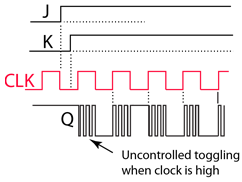
\includegraphics[width=0.55\columnwidth]{images/jkrace1.png}
    \caption{Diagram depicting JK racing when the clock is high}
    \label{race0}
\end{figure}

% =====================================================================================
\subsection*{Master-Slave JK Flip-flop}
To avoid racing in the JK flip-flop, the timing pulse period must be kept as short as possible, which is not very practical with modern TTL IC's. A Master-slave JK solves this problem by using two SR flip-flops connected in series -- the \textit{master circuit}, which triggers the leading edge of the clock pulse and the \textit{slave circuit}, which triggers the falling edge of the clock pulse. Hence the uncontrolled toggling is suppressed as the transmission of the J value to the output is delayed by half a clock cycle and not immediately fed back to the input side.

\begin{figure}[H]
    \centering
    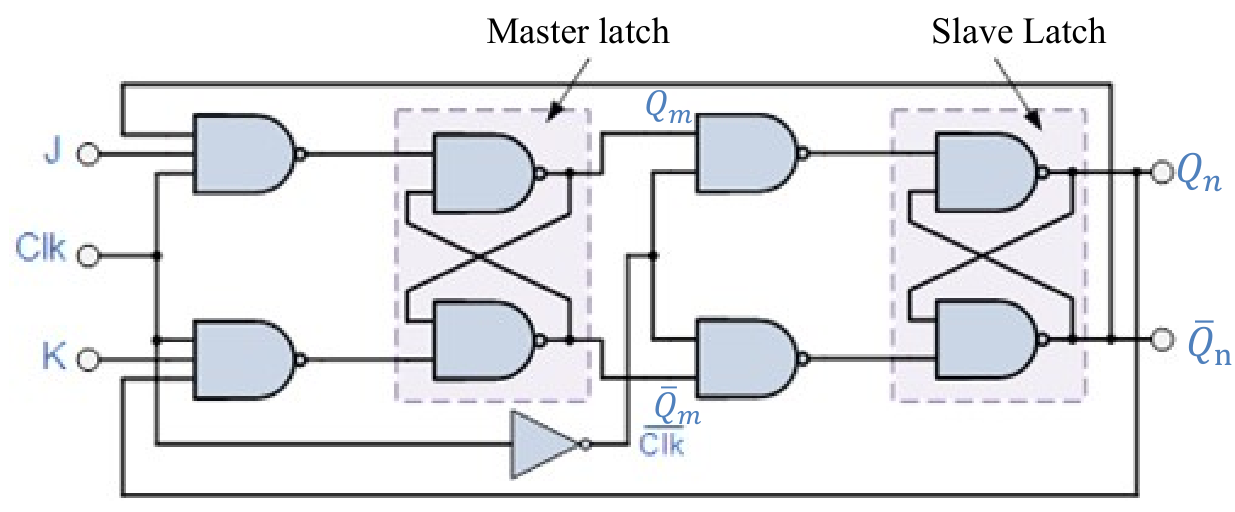
\includegraphics[width=0.90\columnwidth]{images/msjk.png}
    \caption{Circuit diagram of a Master-slave JK flip-flop}
    \label{5}
\end{figure}

When a clock pulse enables the master flip-flop, it disables the slave flip-flop (as its clock signal is inverted). When the clock
changes state again (i.e., on its falling edge) the output of the master latch is transferred
to the slave latch. Again, toggling is accomplished by the connection of the output with
the input AND gates.

\begin{table}[H]
    \centering
    \begin{tabular}{|c|c|c|c|c|c|c|}\hline
        CP &$J$ & $K$ & $Q_m$ & $ Q'_m$ & $Q_n$ & $ Q'_n$ \\ \hline
        $0 \rightarrow 1$ & 0 & 0 & \multicolumn{2}{c|}{Hold} & \multicolumn{2}{c|}{Hold} \\ \hline
        $1 \rightarrow 0$ & 0 & 0 & \multicolumn{2}{c|}{Hold} & \multicolumn{2}{c|}{Hold} \\ \hline
        $0 \rightarrow 1$ & 0 & 1 & 0 & 1 & \multicolumn{2}{c|}{Hold} \\ \hline
        $1 \rightarrow 0$ & 0 & 1 & \multicolumn{2}{c|}{Hold} & 0 & 1 \\ \hline
        $0 \rightarrow 1$ & 1 & 0 & 1 & 0 & \multicolumn{2}{c|}{Hold}\\ \hline
        $1 \rightarrow 0$ & 1 & 0 & \multicolumn{2}{c|}{Hold} & 1 & 0\\ \hline
        $0 \rightarrow 1$ & 1 & 1 & \multicolumn{2}{c|}{Toggle} & \multicolumn{2}{c|}{Hold} \\\hline
        $1 \rightarrow 0$ & 1 & 1 & \multicolumn{2}{c|}{Hold} & \multicolumn{2}{c|}{Toggle} \\ \hline
    \end{tabular}
    \caption{Characteristic Table for a Master-slave JK Flip-flop}
\end{table}

\begin{figure}[H]
    \centering
    
\includegraphics[width=1\columnwidth]{images/jkrace3.png}
    \caption{The output changes once in a clock cycle in case of a master-slave JK flip-flop. This solves the racing problem in a single stage JK flip-flop.}
    \label{race}
\end{figure}
% =====================================================================================
\subsection*{T Flip-flop}
T or Toggle flip-flop is a modification on the master-slave JK flip-flop where it only performs toggling action. Here, we make $J=K=1$.
\begin{itemize}
    \item When Clk $=0$, the state will be stored (\verb|HOLD|) regardless of the value of T.
    \item When Clk $=1$ and $T=0$, the previous state is stored, i.e. \verb|HOLD| state.
    \item When Clk $=1$ and $T=1$, we will have toggle action.\\
\end{itemize} 

\begin{table}[H]
    \centering
    \begin{tabular}{|c|c|c|c|}\hline
        $Q_N$ & $T$ & $Q_{N+1}$ & Remark\\ \hline
        0 & 0 & 0 & \verb|HOLD| \\ 
        0 & 1 & 1 & \verb|TOGGLE| \\ 
        1 & 0 & 1 & \verb|HOLD| \\ 
        1 & 1 & 0 & \verb|TOGGLE|\\ \hline
    \end{tabular}
    \caption{Characteristic Table for a T Flip-flop, where Clk $=1$}
\end{table}
% ======================================================================================
\section{Apparatus}

\begin{enumerate}
    \item ICs (NOR-7402, AND(2-input)-7408, NAND(3-input)-7410, NAND-7400, NOT-7404)
    \item Resistors (1 k$\Omega$)
    \item DC Power Supply (5V)
    \item LEDs
    \item Connecting Wires
    \item Multimeters
\end{enumerate}